\section{Methods}
\label{sec:methods}



\subsection{Persistent Homology}
\label{sec:persistence}
%\todo{Bala to write this part}

The input to the persistent homology (PH) pipeline \cite{edelsbrunner_persistent_2013} is a high dimensional point cloud $\mathcal{X}$ of $n$ points in $d$ dimensions with a distance $\mathrm{dist}(x,y)$ specified for any pair $x,y \in \mathcal{X}$.
In short, PH characterizes the structure of $\mathcal{X}$ by identifying features in each dimension that persist across multiple scales of $\mathrm{dist}$ values.
It tracks a simplicial complex $K$ built on $\mathcal{X}$ as a function of distance values $\mathrm{dist} \leq r$ for $r \geq 0$.
At any given cutoff $r$, an edge $xy \in K$ when $\mathrm{dist}(x,y) \leq r$.
Similarly, a triangle $xyz \in K$ when every pairwise $\mathrm{dist}$ for points $\{x,y,z\}$ is $\leq r$, and so on.
PH then tracks the evolution of algebraic objects (groups) defined on $K$ as $r$ increases.
It creates a \emph{persistence diagram} (PD) $\mathrm{dgm}_i$ in dimension $i$ that represents each $i$-dimensional feature by a point in the 2D plane with coordinates $\langle$birth,death$\rangle$ corresponding to the values of $r$ at which the feature starts and one at which it stops existing.
In particular, $\mathrm{dgm}_0$ captures the evolution of connected components, while $\mathrm{dgm}_1$ captures the evolution of \emph{holes} in $\mathcal{X}$.
In this work, we concentrate on $\mathrm{dgm}_1$ PDs as holes in $\mathcal{X}$ can be used to capture branching behavior (see Section~\ref{sec:PDforCH}).  

Furthermore, the PH pipeline provides a natural way to compare pairs of data sets $\mathcal{X}$ and $\mathcal{Y}$ based on their branching behavior. 
We first generate the corresponding PDs $\mathrm{dgm}_1(\mathcal{X})$ and $\mathrm{dgm}_1(\mathcal{Y})$.
Considering these PDs as histograms (or probability measures), we compute the \emph{Wasserstein distance} $\mathrm{WD}(\mathrm{dgm}_1(\mathcal{X}), \mathrm{dgm}_1(\mathcal{Y}))$ between them (also known as the Earth mover's distance).
We then use the WD values to directly compare the data sets $\mathcal{X}$ and $\mathcal{Y}$.

%\delete{
%- Persistent homology intro with notation\\
%- how to find H0 and H1 explanation\\
%- Holes could be used to detect branching events as we show. \\
%- transformation (normalization) to make different oblong loops into more circular loops so that we can detect them invariant to the scale of the different dimensions
%- can talk about appropriate definition of $\mathrm{dist}$ as justification of our normalization(s) 
%}
\begin{figure*}[tbh!]
\centering
%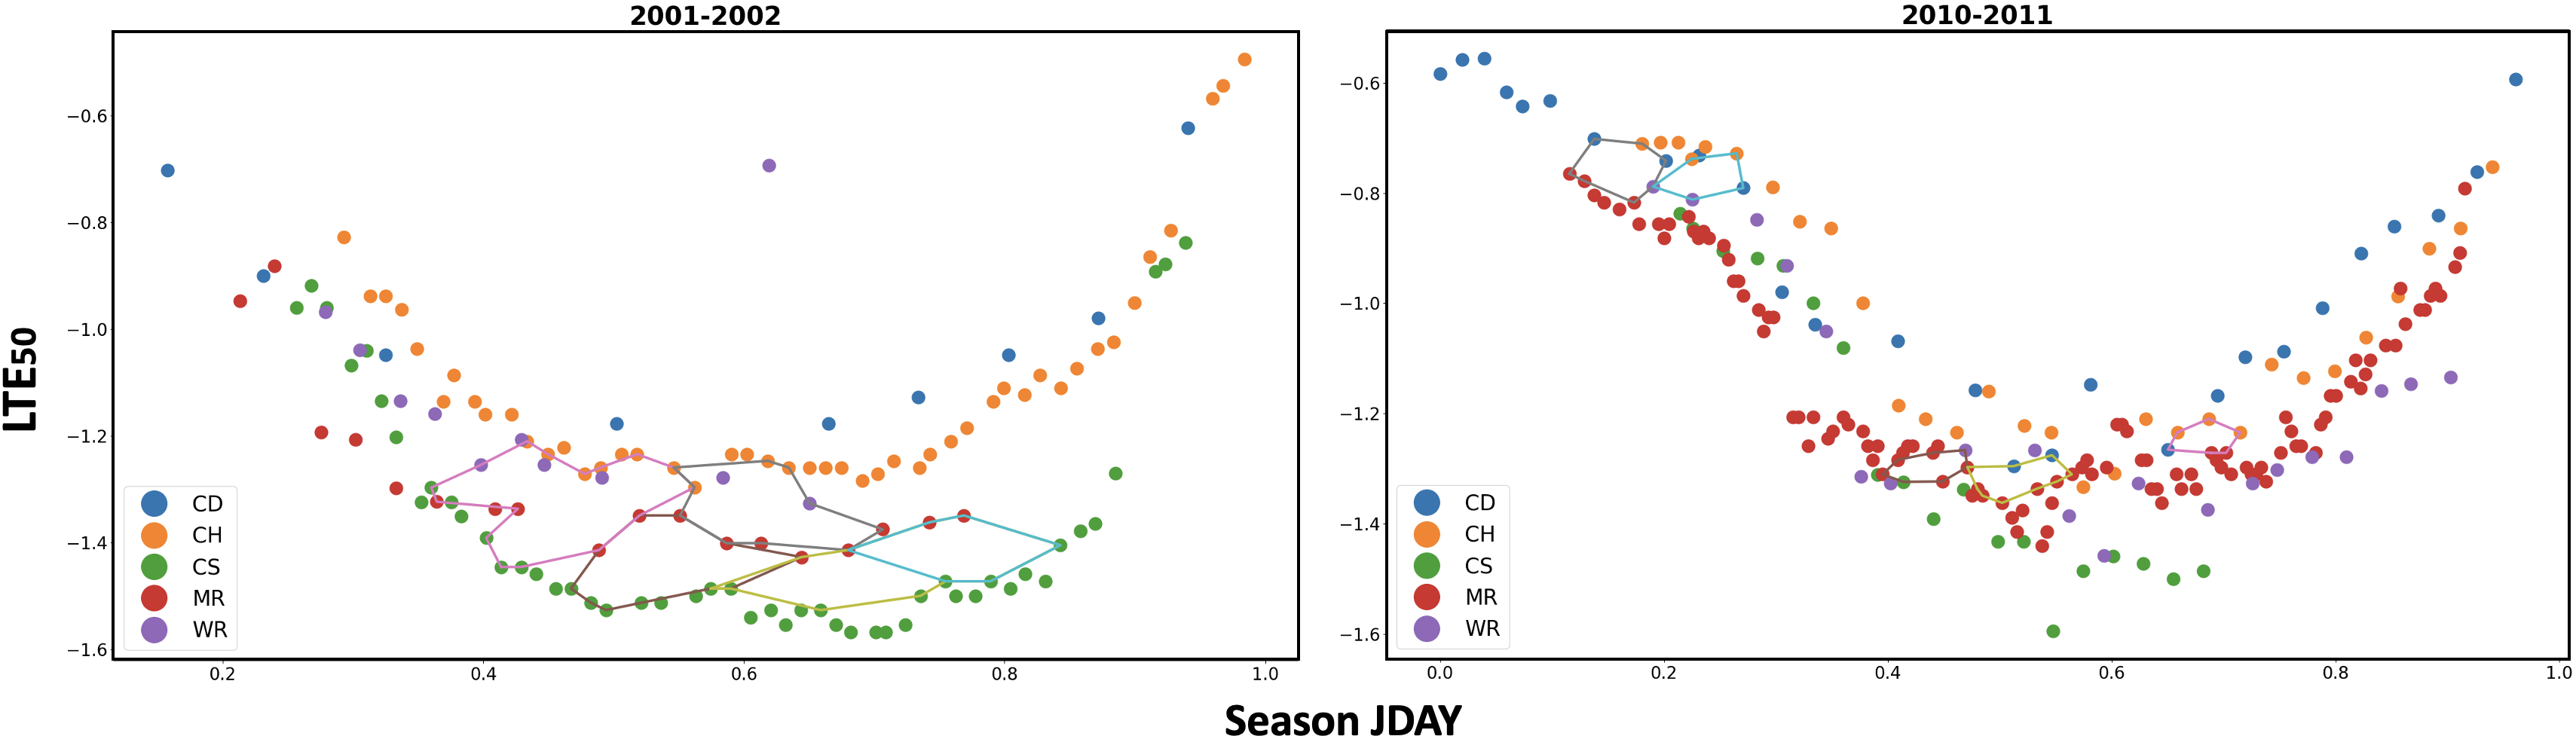
\includegraphics[width=2.1\columnwidth]{Figures/HolesSeason.png} 
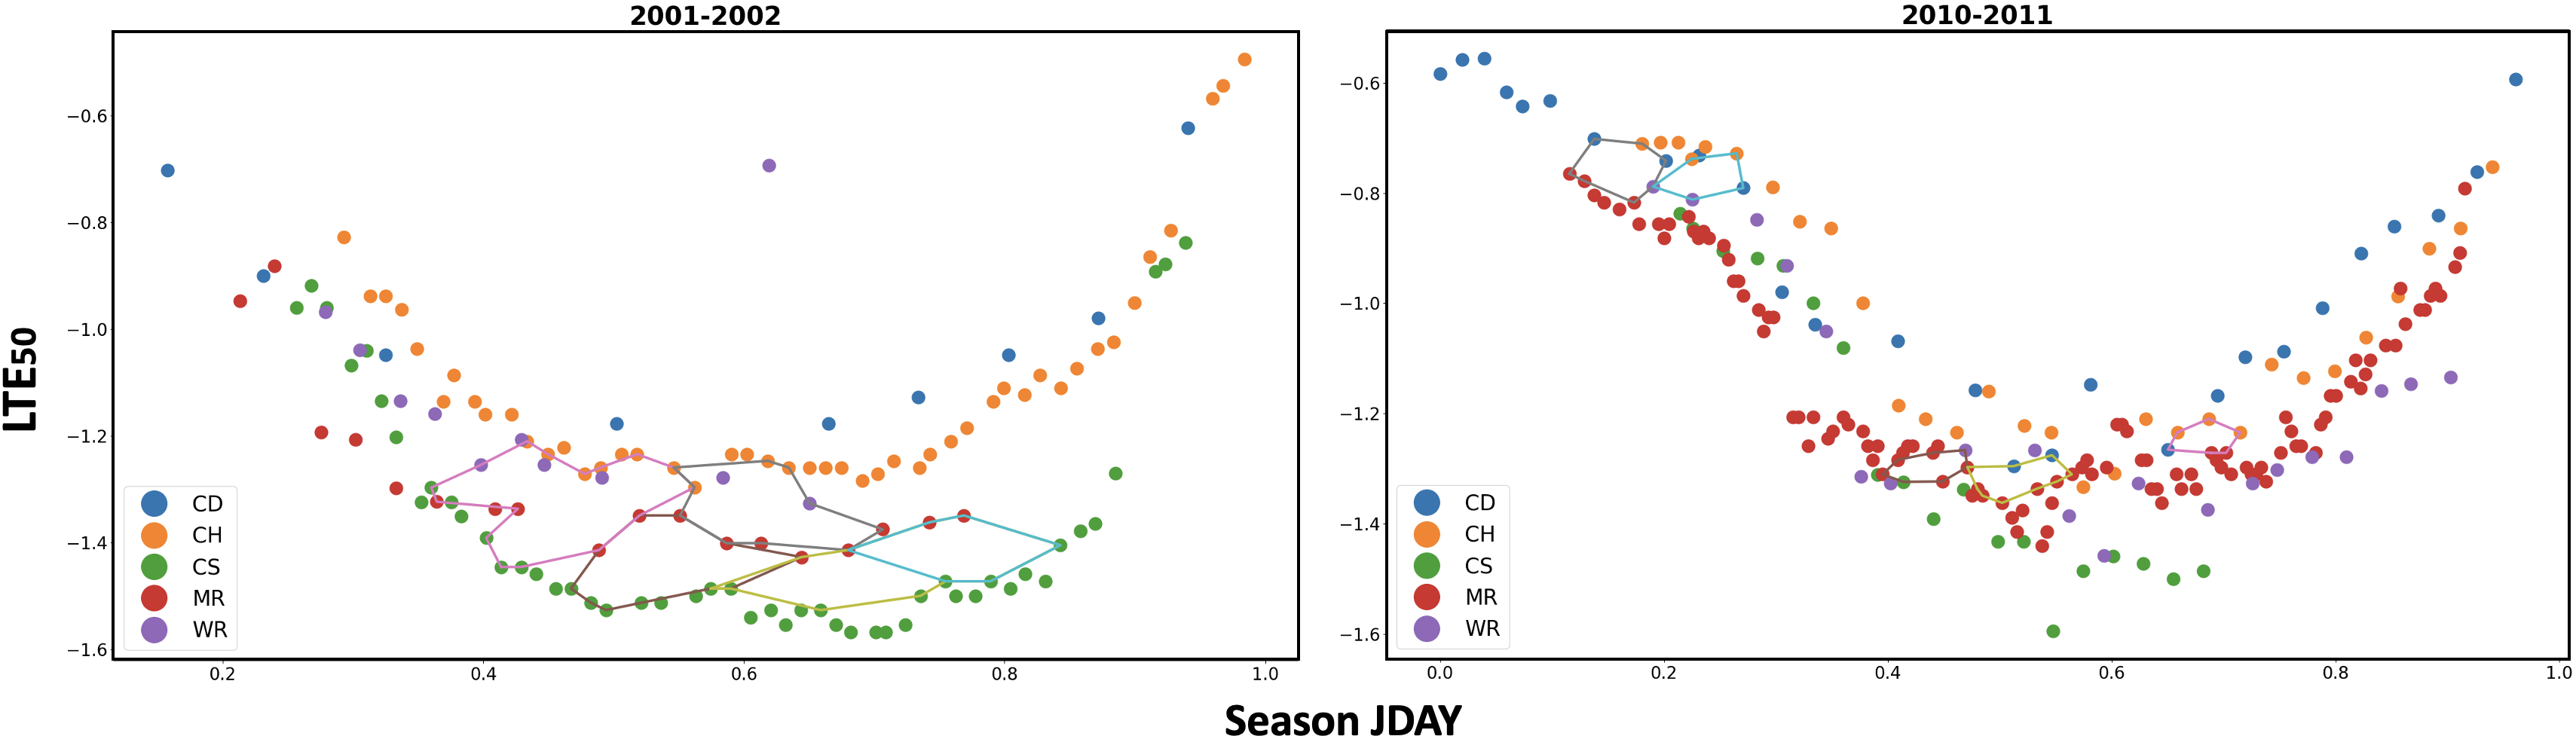
\includegraphics[scale=0.25]{Figures/HolesSeason.png} 
\caption{Branching events detected by persistent homology for each point cloud data set. 2001-2002 and 2010-2011 were the pair with the greatest Wasserstein Distance for their respective persistence diagrams among all season pairs.
The y-axis LTE value is calculated using Eqn.~(\ref{eqn:norm}).
}
\label{fig:holesseason}
\end{figure*}

\subsection{Building Persistence Diagrams for Analyzing Cold Hardiness Behavior}
\label{sec:PDforCH}


In the case of cold hardiness, each point in the point cloud $\mathcal{X}$  is a 4-tuple 
$\langle c, s, d, h \rangle$, where $c$ is the cultivar label, $s$ is the season/year, $d$ is a JDAY of the season, and $h$ is the cold hardiness value (i.e., the phenotype) observed that day for that cultivar, which is one of $LTE_{10}$, $LTE_{50}$, or $LTE_{90}$.


Using this input point cloud $\mathcal{X}$, we construct different types of persistence diagrams (Section~\ref{sec:persistence}) to answer different kinds of queries as described below. 

\paragraph{Task 1. Computing Inter-cultivar and Intra-cultivar relationships.}
Consider two cultivars $c_1$ and $c_2$ that exhibit similar LTE values during most of the season except for an interval when they diverge in their values. It is also possible that such divergent behavior may be observable at  multiple time scales---e.g., two cultivars could diverge for days, while another two cultivars could diverge for weeks to months. 

Furthermore, it is  possible the LTE behavior exhibited by a single cultivar across two different seasons is divergent. For instance, a cultivar $c$ may exhibit a higher range of LTE values during one season and a lower range in another season, both during the same JDAY time interval. 

In what follows, we present an approach using persistence diagrams to detect these distinct kinds of divergent behavior.  

\begin{compactenum}[S1)]
\item 
For each cultivar $c$, construct a point cloud $\mathcal{X}_c\subseteq \mathcal{X}$ with all points of the form $\langle d,h \rangle$ taken from all points in $\mathcal{X}$ corresponding to cultivar $c$.
\item
Next, for each cultivar $c$ and using $\mathcal{X}_c$, build a persistence diagram containing $\mathrm{dgm}_0$ (connected components) and $\mathrm{dgm}_1$ (holes) as described in Section~\ref{sec:persistence}. We denote those diagrams for cultivar $c$ as $\mathrm{dgm}_0^c$ and $\mathrm{dgm}_1^c$, respectively.
\item 
We then compare each pair of cultivars by computing the pairwise Wasserstein distance (described in Section~\ref{sec:persistence}) between their respective diagrams.
More specifically, for a cultivar pair $c$ and $c'$, we compute 
$\mathrm{WD}(\mathrm{dgm}_1^{c}(\mathcal{X}_{c}),\mathrm{dgm}_1^{c'}(\mathcal{X}_{c'}))$.
\end{compactenum}

The $\mathrm{dgm}_1$ outputs of step S2 can be used to infer intra-cultivar variability, and the outputs of step S3 to infer inter-cultivar relationships.
Consider a hole detected as part of a $\mathrm{dgm}_1^c(\mathcal{X}_c)$, and let that hole span from day $i$ to day $j$ along the JDAY dimension of the point cloud.
This is indicative of a branching event that starts around day $i$ and ends around day $j$. If the two branching paths are comprised of points from two different seasons $s_1$ and $s_2$ (to be expected), then we infer that the cultivar $c$ shows variable LTE behavior between these two seasons for the JDAY interval $[i,j]$.

Note that different $\mathrm{dist}(.)$ can be used for step S2 to compute the persistence diagrams.
In this paper, we first used two different scaling functions for the two dimensions of the point cloud (JDAY, LTE50), and then used the L2 (Euclidean) distance as the function on the scaled points to construct the persistence diagrams.

For JDAY, we used a simple normalization to scale all points in the range of [0,1]. 

For LTE, instead of using their values directly, we modeled the phenotype value by taking the difference between the observed LTE value and the minimum air temperature recorded on that day (we denote this difference $\delta(s,d,h)$ on day $d$ of season $s$ with LTE $h$). Intuitively, this difference is a strong indicator of the degree of risk that the cultivar faces on that day---as the difference shrinks, the cultivar is at a higher risk.
Note that $\delta(s,d,h)$ can be positive or negative (rare).
Subsequently, we normalize the $\delta$ values as:
\begin{equation}\label{eqn:norm}
\hspace*{-0.05in}
\overline\delta(s,d,h) \hspace*{-0.02in} = \hspace*{-0.02in}
\frac{\delta(s,d,h)-\min_d\{|\delta(s,d,h)|\}\,}{\max_d\{|\delta(s,d,h)|\}-\min_d\{|\delta(s,d,h)|\}} 
\end{equation}
Intuitively, this normalization function is aimed at making an oval or oblong branching shape into a more circular shape, making it suited for hole detection (examples shown in Figure~\ref{fig:holesseason}).


%\SW{Transformation formula: df['LTE50'] = (df['LTE50'] - df['LTE50'].abs().min()) / (df['LTE50'].abs().max() - df['LTE50'].abs().min())}


\paragraph{Task 2. Computing seasonal correlations.}
Given multiple seasons, we are also interested in computing pairwise seasonal correlations. Two seasons are said to be \emph{similar} if all the cultivars considered show consistent relative behavior between the two seasons. 
There are two ways to compute this relationship. 
We can directly compare the point clouds for those two seasons. 
Alternatively, we can build the persistence diagrams for those two seasons and compare them. 
We choose the latter approach since persistence diagrams are more compact representations with robust properties \cite{edelsbrunner_persistent_2013}.


